\chapter{Background}
\label{chpt:2}
\paragraph{}
This chapter provides an overview of the different task and concepts needed to perform relation extraction in a multilingual setup. Some concepts, like Word Representation~(Section \ref{sec:word_embedding}) are at the core of NLP, while others are more general machine learning techniques (Section~\ref{sec:nn},~\ref{sec:transfer_learning} and \ref{sec:zero_learning}), some others instead are both general and have a very high usage in NLP due to their nature (Section \ref{sec:sequence_modeling}). After a brief description of each of these concepts, we will focus on their application in NLP in particular for relation extraction. In the next Chapter we will describe more the task of relation extraction, and present how Natural Language Understanding, a sub-field of NLP that deals with machine reading comprehension, can be used for relation extraction.

% \section{Introduction}
% Natural Language Processing solutions span form rule based systems~\citep{brill-1992-simple, nebhi2013rulere}, to statistical approaches~\citep{skounakis2003hierarchical}, and also to neural networks~\citep{pawar-etal-2017-end}.

\section{Neural Networks}
\label{sec:nn}

\paragraph{}
A Neural Network (NN) is a computational model inspired by networks of biological neurons, wherein the neurons compute output values from inputs. The simplest form of neural network is the feed forward neural network, in which the information flows only in one direction, and there is no recurrent connection between the nodes. Neural networks try to approximate some function $f^{*}$ by defining a mapping $y = f(x; W)$ for an input $x$ and learning the value of the parameters $W$ that yield the best function approximation. A neural network is called network because they contain multiple layers of artificial neurons. The artificial neuron is the building block of neural networks.

A neuron is defined by an input $x$, a set of weights $W$, a bias $b$, and an activation function $g$. The activation function should be differentiable, since to actually learn, we need to compute derivatives. With $x, W \in \mathbb{R}^{n\times1}$, $b \in \mathbb{R}$. The output $y$ is defined as: 

\begin{equation}
    y = g(W^{\intercal} x + b)
\end{equation}


Feed forward neural networks are composed by various layers, each layer contains some neurons. The formal definition is very similar to the one of the neuron. We will include the bias term in the weights matrix, and have an extra element $x_0 = 1$ in the input $x$. Given a feed forward neural network with $L$ layers, the forward propagation is: 

\begin{equation}
\begin{split}
    %y = f^{k}(W_{k}^{\intercal} * \dots f^{2}(W_{2}^{\intercal} * f^{1}(W_{1}^{\intercal} * x)) \dots)
    z & = W^{i-1}a^{i-1} \\
    a^{i} & = g(z^i) \\
    y & = a^L g(z^L) \\
\end{split}
\end{equation}

Where $g$ is an activation function, $a^i$ is the activation of layer $i$, and $a^0 = x$. The weight matrix $W_i$ controls the mapping from layer $i$ to layer $i+1$. Given a network with $s_i$ units in layer $i$, and $s_{i+1}$ in layer $i+1$ the weight matrix $W_i \in\mathbb{R}^{(s_{i+1})\times (s_i + 1)} $. And the final prediction is $y = a^{L}$. 

As in other machine learning algorithms, we have to learn the parameters of our neural network. We have a cost function, or objective function, $J(\theta)$ that we try to minimize. Given a neural network $h_\theta$, we compute our cost function as a sum of the error function  $\mathcal{L}$ for all the examples. The error function computes the difference between the predicted value $\hat{y} = h_{\theta}(x)$ and the actual value $y$. We also have a regularizer term $\Omega$ that is weighted by the hyperparameter $\lambda$:

\begin{equation}
    \min_{\theta} J(\theta) = - \frac{1}{N} \sum_{1}^{N} \mathcal{L}(y_i, \hat{y_i}) + \lambda \Omega_\theta
\end{equation}

Now that we have defined what is the goal of our neural network, we can start performing the training. %The learning algorithm for neural network is called backpropagation, from backward propagation of errors. 
The weights $\theta$ in the network are the only parameters that can be modified to make the cost function $J$ as low as possible; thus we can minimize $J$ by using an iterative process of gradient descent, for which we need to calculate the gradient for the cost function with respect to the network parameters.  As each network consists of various layers, computing the gradient of the loss function w.r.t the parameters $\frac{\partial J}{\partial \theta}$ is non-trivial. To estimate the gradient, we use a an algorithm called backpropagation~\citep{rumelhart1988learning}, from backward propagation of errors. As the name implies, backpropagation starts computing the gradients from the output of the networks and moves backward to the input through all layers. First, we need to compute the derivative of $J(\theta)$ w.r.t the output, this will be our $\partial^{L}$, then go backward:



%Equation~\ref{eq:backpropagation}. 

\begin{equation}
\begin{split}
    \partial^{L} & = \frac{\partial}{\partial y} \mathcal{L}(y, \hat{y}) \\
    \partial^i &= {\theta^{i}}^\intercal \partial^{i+1} \odot \left(\frac{\partial}{\partial z^{i}} g(z^i)\right)
\end{split}
\label{eq:backpropagation}    
\end{equation}

For each layer, the computed gradients are then used to update the corresponding parameters using gradient descent.

\section{Sequence Modeling}
\label{sec:sequence_modeling}


\paragraph{}
Due to the inherent nature of natural language almost all NLP tasks deal with sequences. For example, in speech recognition, we have the input audio which is a sequence of phonemes that will be recognised and used to produce a transcript. Likewise, in machine translation where we have as input a sequence of words in a source language and the machine has to generate a sequence of words with the same meaning of the one in input but in a target language.


Traditional neural networks are not designed to deal with the temporal information of sequences in an efficient way. A way to handle this problem is to introduce the notion of a dynamical system. In the dynamical system, there is a state which carries information about past inputs. Typically, we make what is called a Markov assumption; that means that all the information regarding the past and current inputs required to estimate a future state is succinctly contained in the current state. A Recurrent Neural Network is a particular type of dynamical system.

\subsection{Recurrent Neural Network}
\paragraph{}
The most elementary neural network for sequential input is the recurrent neural network~\citep{elman1990finding}. Elman proposes a recurrent network based on the idea introduced by~\citet{jordan1986} which proposes a network with recurrent connections from the output to the input; these are one-to-one connections that are used to associate a static pattern with a serially ordered output pattern. Elman modifies the network by moving the recurrent connection. Instead of having the output connected with the input, Elman adds additional units at the input level, these units are called ``\textit{context units}'' are connected to the hidden layer. Context units are also “hidden” in the sense that they interact exclusively with other nodes internal to the network, and not the outside world. 

In Figure~\ref{fig:rnn} we can have a look at how a RNN works. The network $A$ takes in input $x_t$ and produces an output $h_t$, a loop enables the information to flow from the previous step to the current, allowing the prediction to be affected by the last state of the network. A more effective way to think about RNNs is by unrolling them (right side of Figure~\ref{fig:rnn}). We can formally define $A$ as:

\begin{figure}[t]
        \centering
        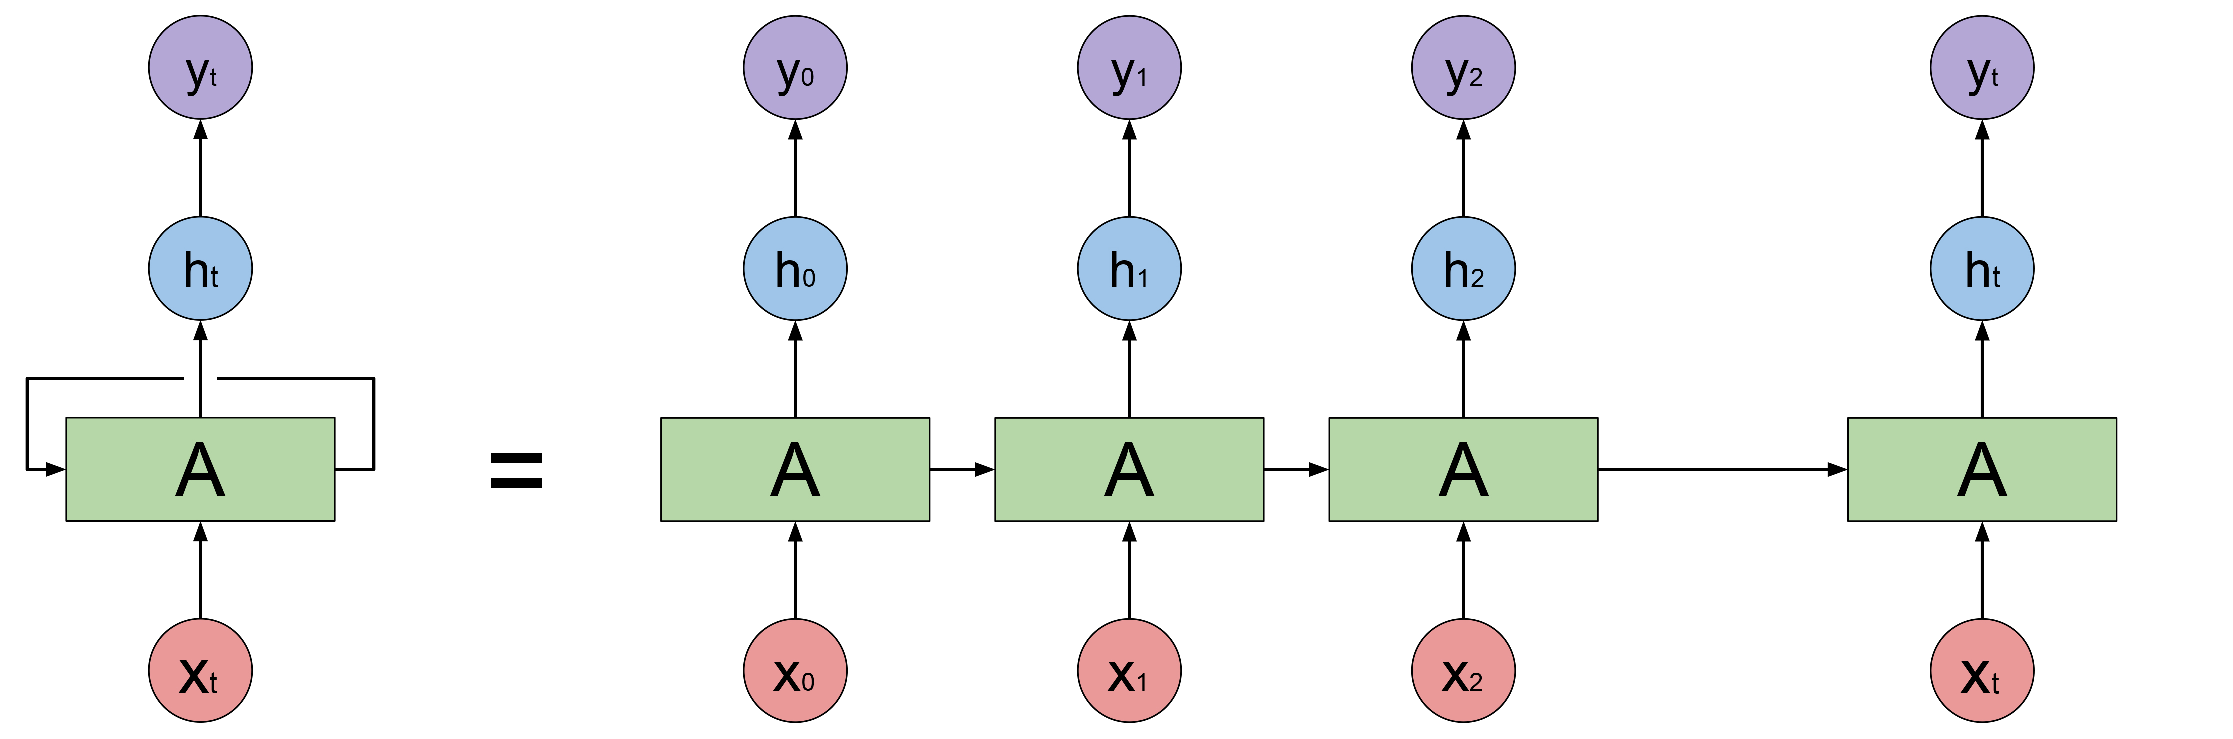
\includegraphics[width=0.9\textwidth]{images/RNN_with_prediction.pdf}
        \caption{RNN unrolling. On the left a compact representation of RNNs, on the right the same RNN can be unrolled}
        \label{fig:rnn}
\end{figure}%

\begin{equation}
\begin{split}
    h_t & = f_W(h_{t-1}, x_t) \\
    y_t & = g_{\theta}(h_t)
\end{split}
\label{eq:generic_rnn}
\end{equation}

Where, $h_t$ is the new state, $f_W$ and $g_\theta$ are functions with parameters $W$ and $\theta$ respectively, $h_{t-1}$ is the previous state, $x_t$ is the current input, and $y_t$ is the output at the \textit{t-th} step.
The vanilla RNN is defined using a neural network with $\tanh$ as activation function, so we will have:

\begin{equation}
\begin{split}
    h_t & = \tanh\left(W_h \cdot h_{t-1} + W_x \cdot x_t\right)\\
        & = \tanh\left([W_h, W_x] \cdot \begin{bmatrix}
           h_{t-1} \\
           x_t
         \end{bmatrix}\right)\\
         & = \tanh\left(W \cdot \begin{bmatrix}
           h_{t-1} \\
           x_t
         \end{bmatrix}\right)
\end{split}
\end{equation}

Where $W_h$, $W_x$ are weights for the hidden and input respectively. 

\paragraph{}
RNN are able to manage variable length of input and output sequences, we can have different types of RNN according to these sizes. Given a sequence $x$ of length $l_x$, and a desired output sequence $y$ with length $l_y$, we can define the following types (visually represented in Figure~\ref{fig:rnn_types}):

\begin{enumerate}[a), noitemsep]
    \item One-to-One: $l_x = l_y = 1$, this is a traditional neural network;
    \item One-to-Many: $l_x = 1, l_y > 1$, this is the case for sequence generation;
    \item Many-to-One: $l_x > 1, l_y = 1$, for sequence classification;
    \item Many-to-Many: $l_x = l_y > 1$, for sequence labeling;
    \item Many-to-Many: $l_x \neq l_y, l_x > 1, l_y > 1$, also referred to as sequence to sequence~\citep{sutskever2014sequence}, or encoder-decoder~\citep{cho-etal-2014-learning}. Given an input sequence, the encoder process it and generates a dense representation, usually the last hidden state, that is used to initialize the decoder that will produce the output sequence.
\end{enumerate}

\begin{figure}
\begin{tcbitemize}[
    raster columns=3,
    raster halign=center,
    raster every box/.style={blankest}
    ]
\mysubfig{One-to-One}{images/one_to_one.pdf}
\mysubfig{One-to-Many}{images/one_to_many.pdf}
\mysubfig{Many-to-One}{images/many_to_one.pdf}
\mysubfig{Many-to-Many}{images/many_to_many.pdf}
\mysubfig{Many-to-Many}{images/many_to_many_s2s.pdf}
\end{tcbitemize}

\caption{Different types of RNN}
\label{fig:rnn_types}
\end{figure}

% \begin{figure} [H]
% \centering
% \begin{tabular}{cccc}
% 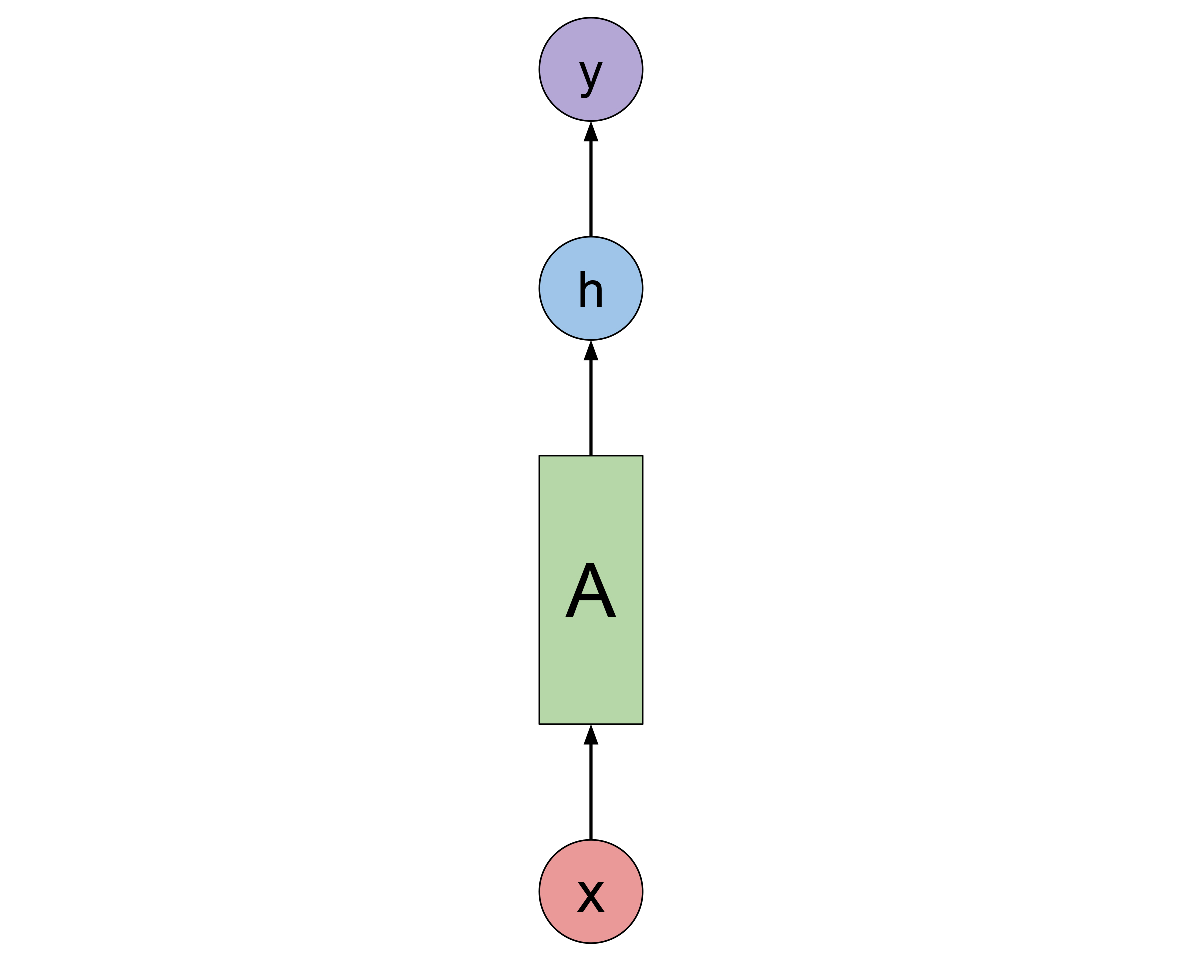
\includegraphics[width=0.3\textwidth]{images/one_to_one.pdf} &
% 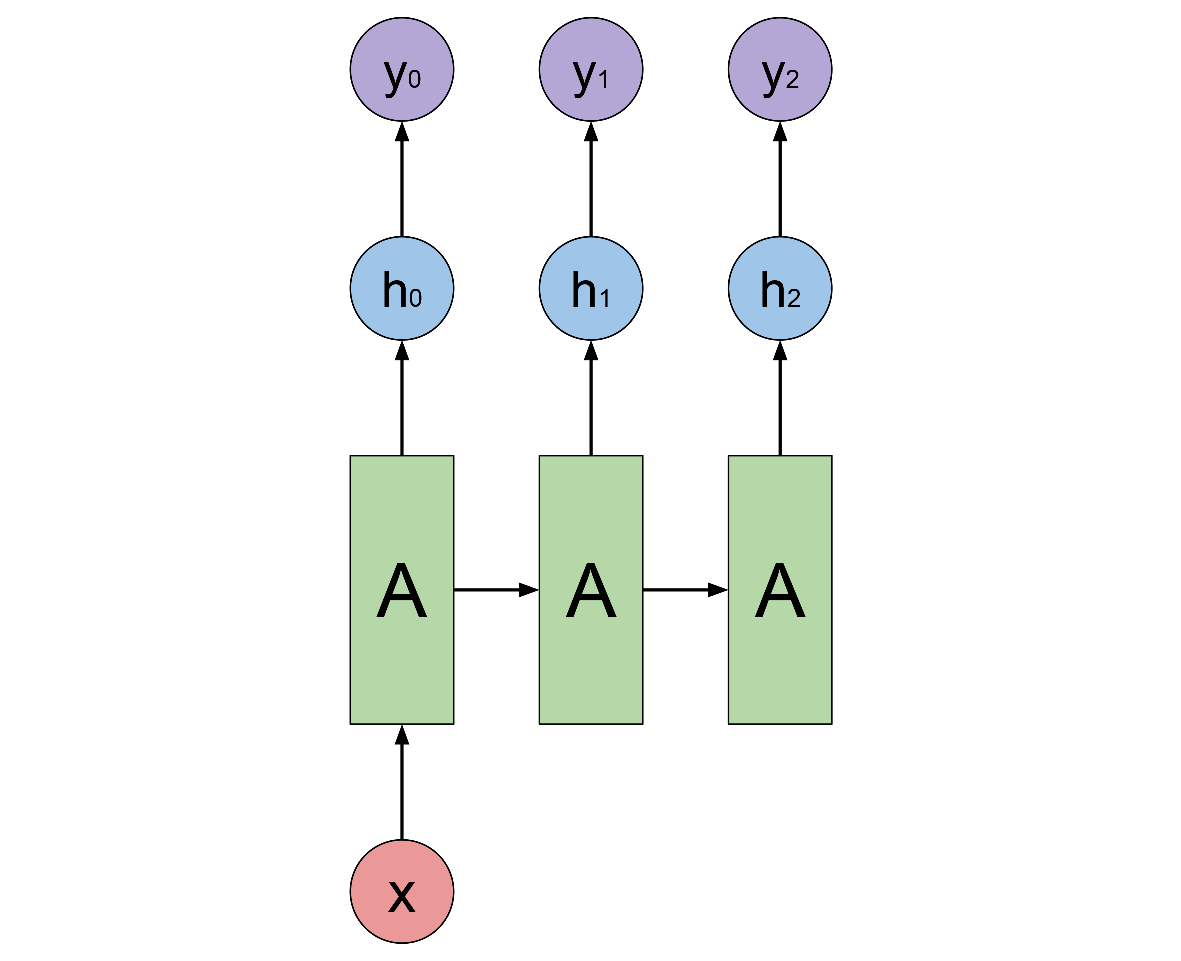
\includegraphics[width=0.3\textwidth]{images/one_to_many.pdf} &
% 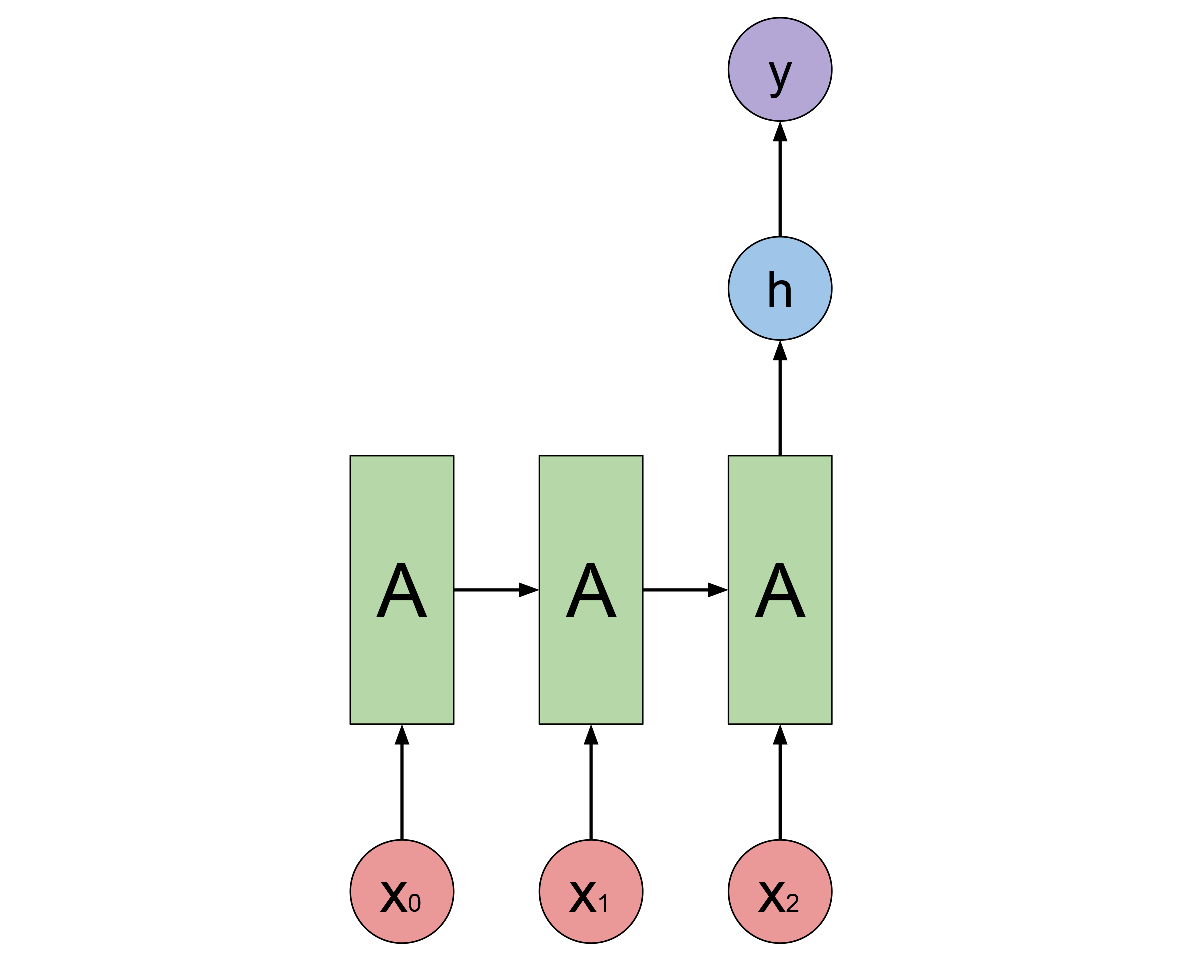
\includegraphics[width=0.3\textwidth]{images/many_to_one.pdf} \\
% \textbf{(a)}  & \textbf{(b)} & \textbf{(c)}  \\[6pt]
% \end{tabular}
% \begin{tabular}{cccc}
% \includegraphics[width=0.3\textwidth]{example-image-a} &
% \includegraphics[width=0.3\textwidth]{example-image-b} \\
% \textbf{(d)}  & \textbf{(e)}  \\[6pt]
% \end{tabular}
% \caption{ \textbf{(a)} Some text
% \textbf{(b)} Some text
% \textbf{(c)} Some text
% \textbf{(a)} Some text
% \textbf{(b)} Some text}
% \label{fig:peroxide}
% \end{figure}

% \begin{table}[ht]
% \caption{A table arranging  images}
% \centering
% \begin{tabular}{*{4}{|m{0.24\textwidth}}|}
% \hline
% 1 & 2 & 3 & 4  \\
% \hline
%  \begin{center}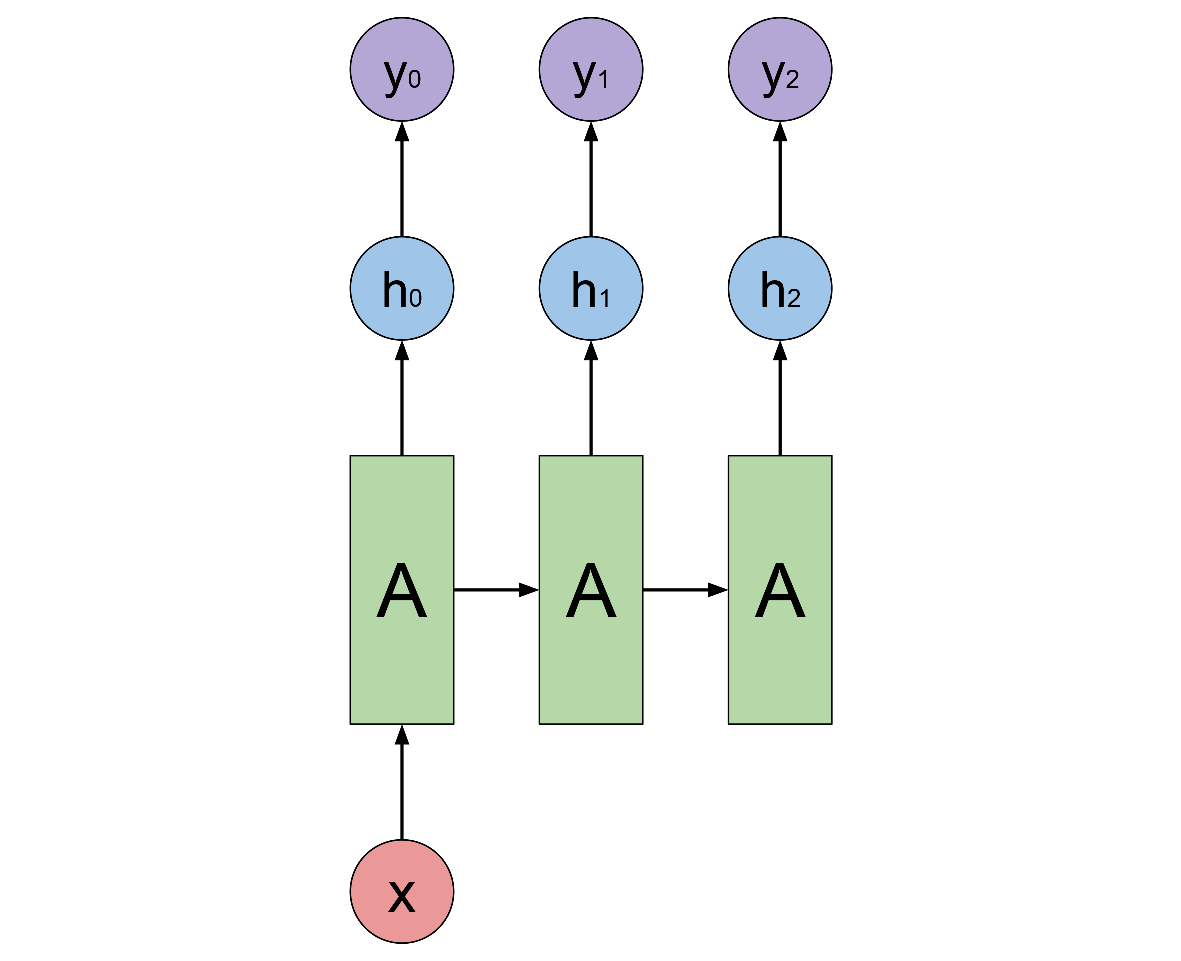
\includegraphics[height=0.1\textwidth]{images/one_to_many.pdf} \end{center} &
% \begin{center}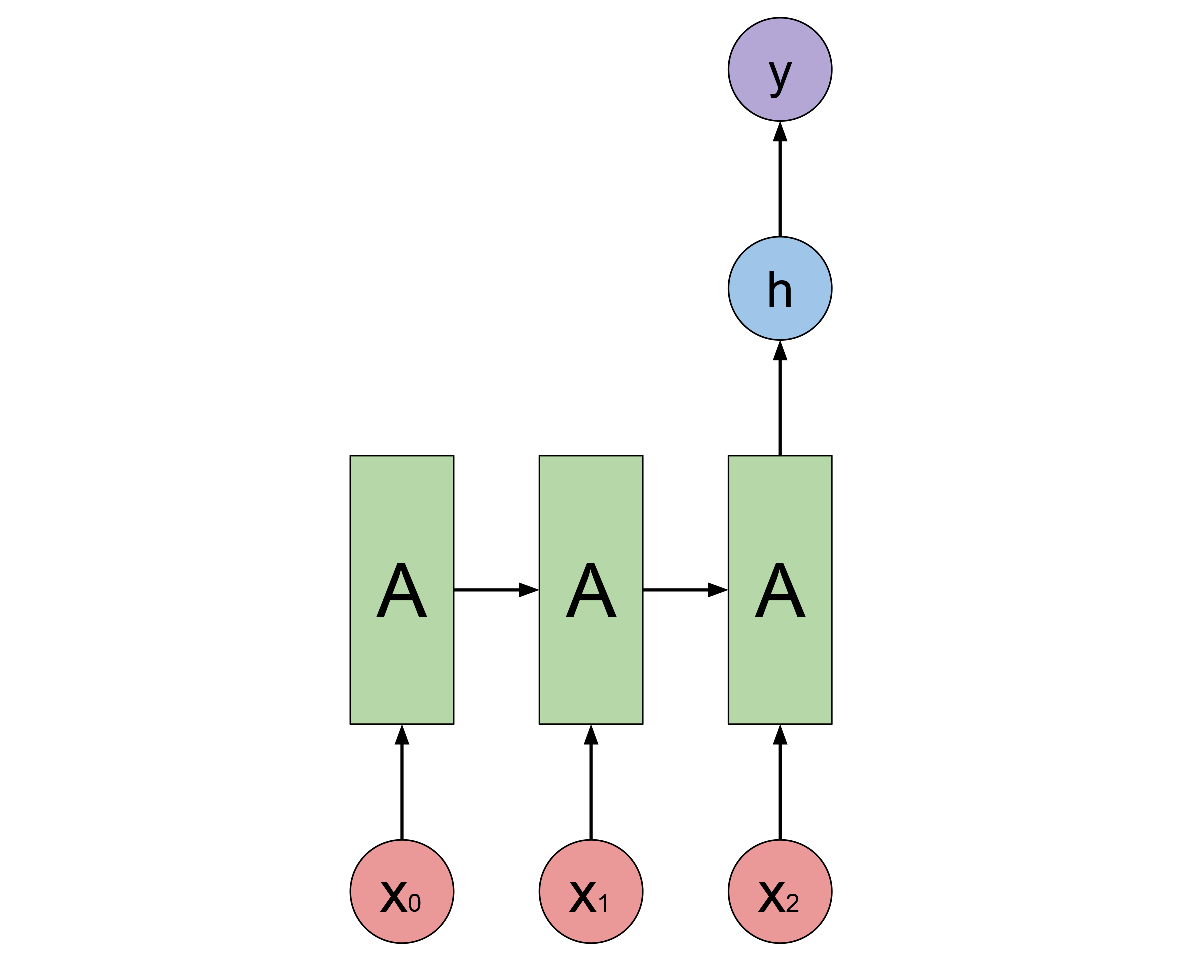
\includegraphics[height=0.1\textwidth]{images/many_to_one.pdf} \end{center} &
% \begin{center}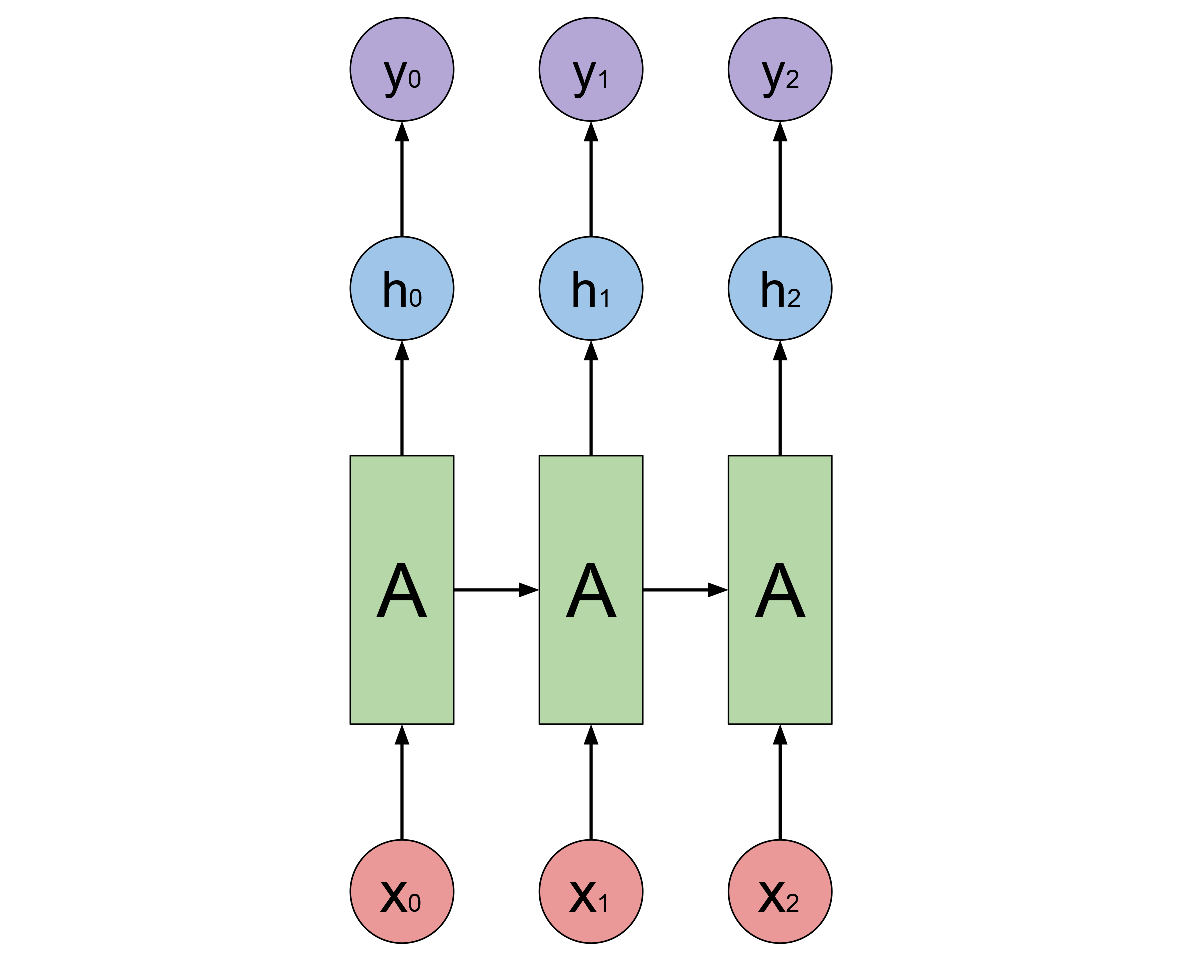
\includegraphics[height=0.1\textwidth]{images/many_to_many.pdf} \end{center} & \begin{center}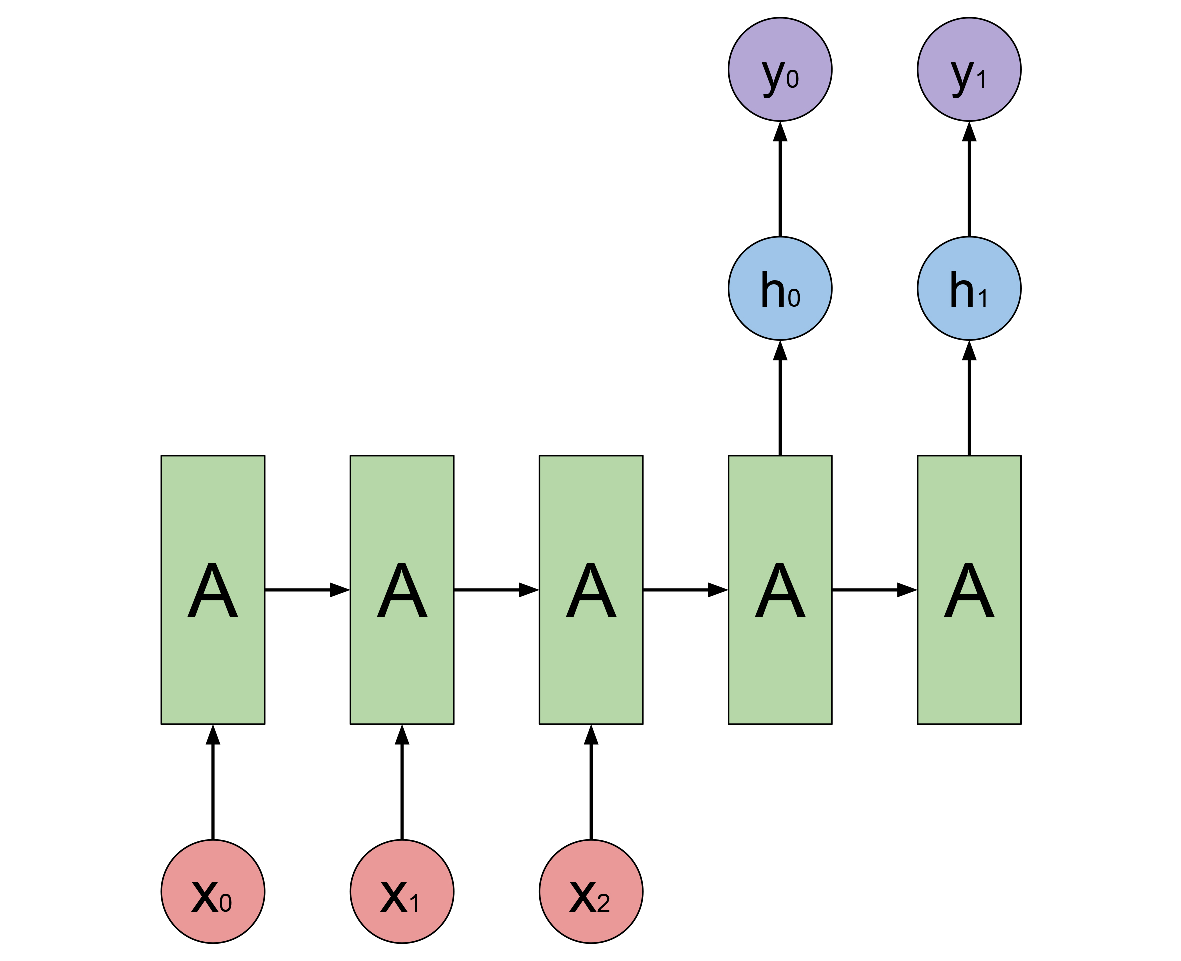
\includegraphics[height=0.1\textwidth]{images/many_to_many_s2s.pdf} \end{center} \\
% \hline
% \end{tabular}
% \label{tab:gt}
% \end{table}

% \begin{table}[ht]
% \caption{A table arranging  images}
% \centering
% \begin{tabular}{*{4}{|m{0.24\textwidth}}|}
% \hline
% This is some text & \begin{center}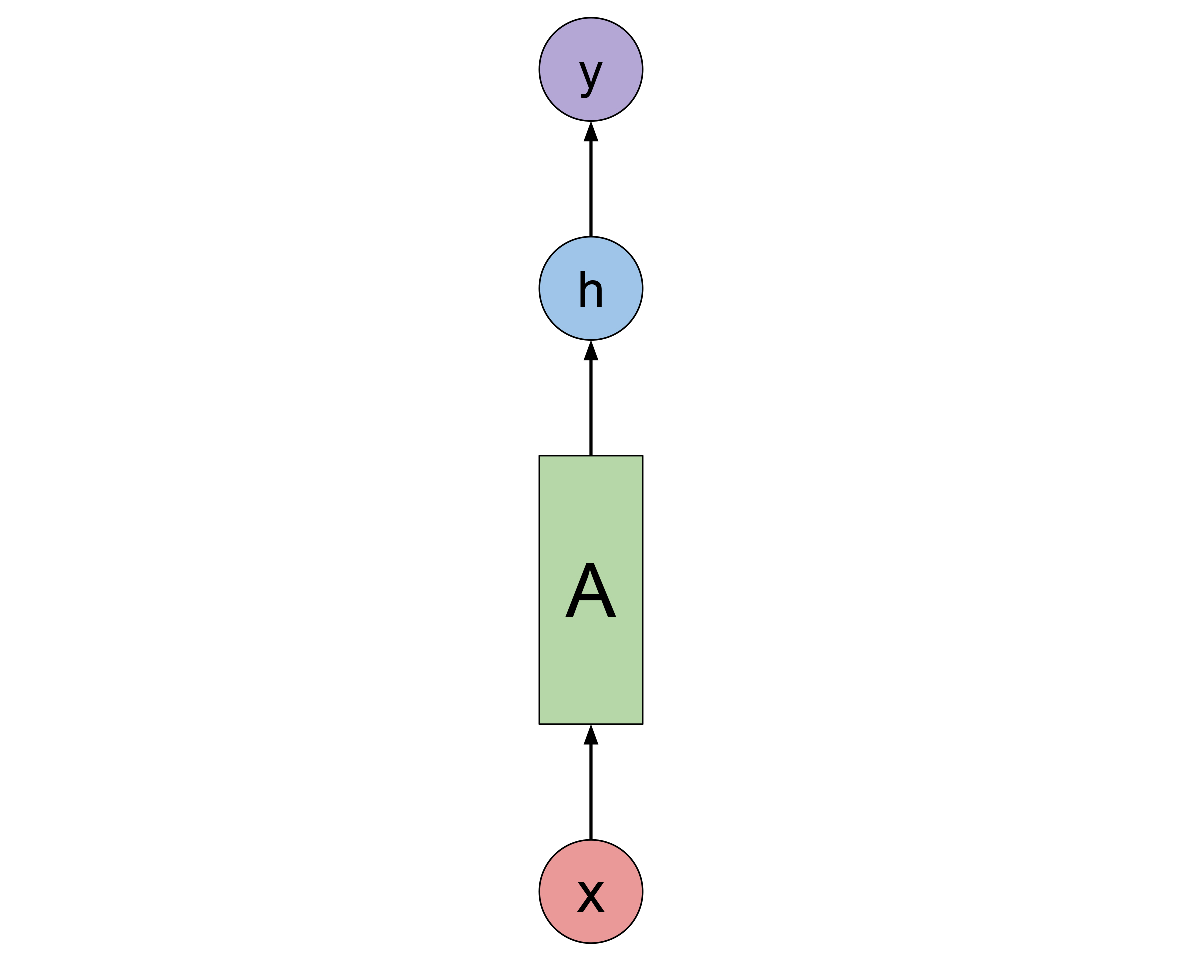
\includegraphics[height=0.2\textwidth]{images/one_to_one.pdf}\end{center} & This is some text & \begin{center}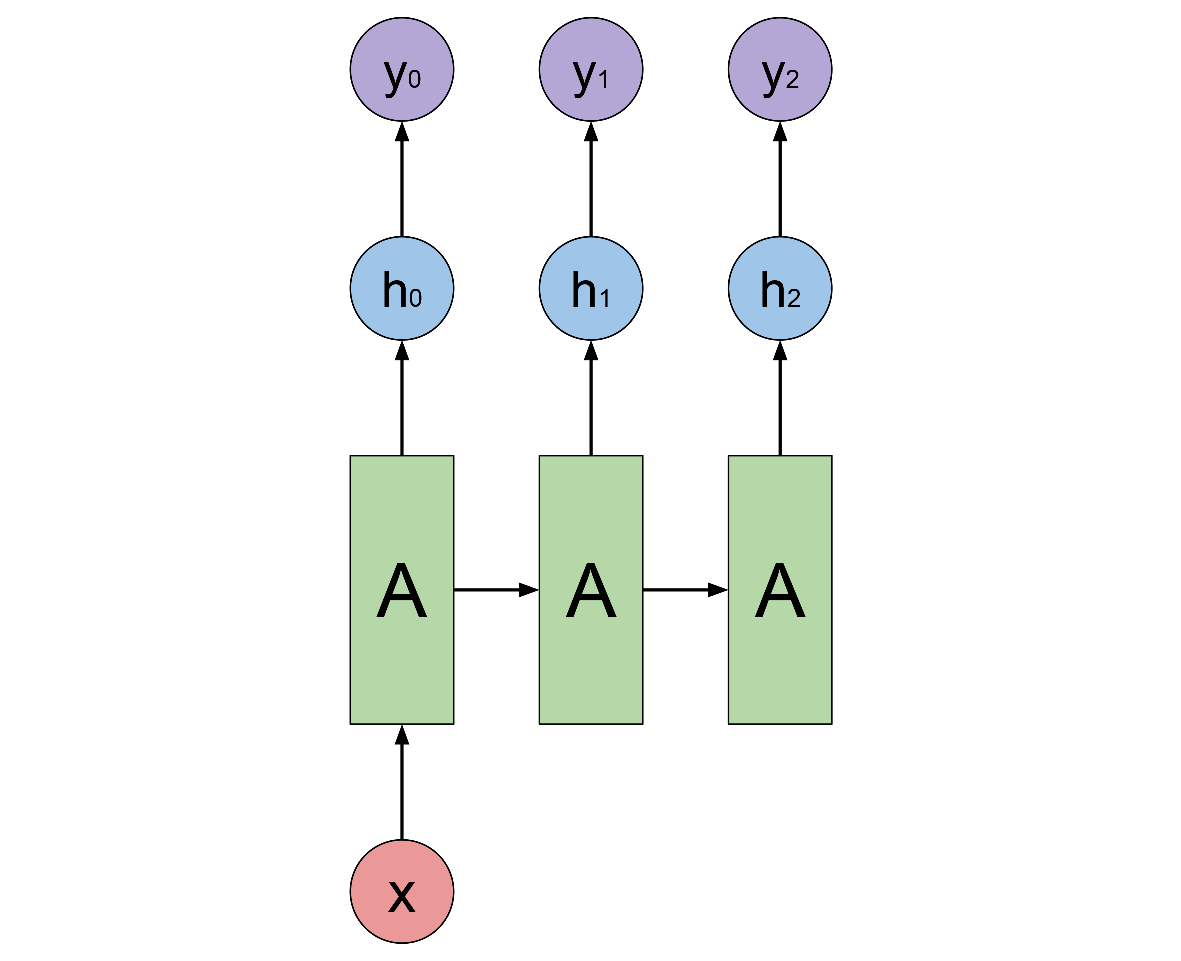
\includegraphics[height=0.2\textwidth]{images/one_to_many.pdf}\end{center} \\
% \hline
% This is some text & \begin{center}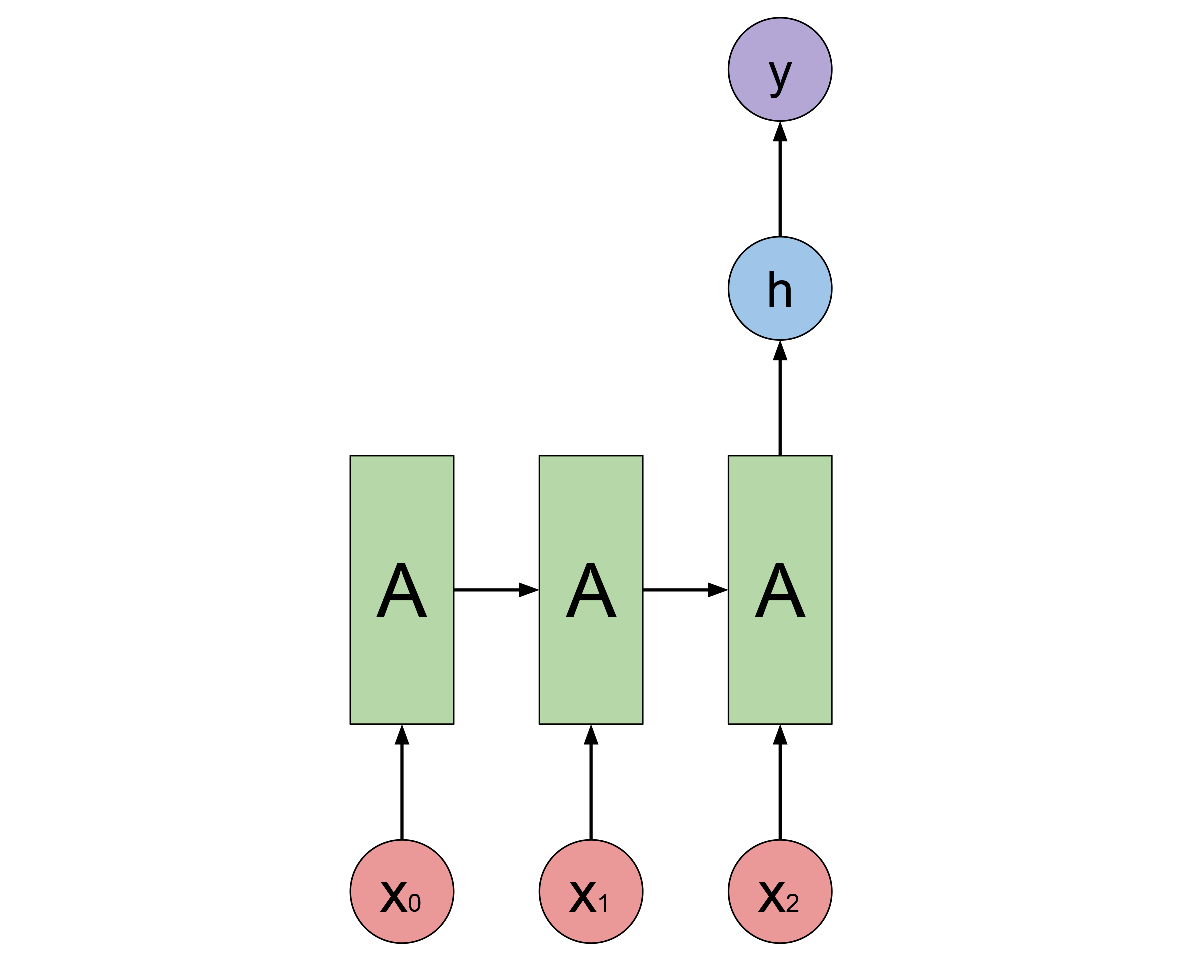
\includegraphics[height=0.2\textwidth]{images/many_to_one.pdf}\end{center} & This is some text & \begin{center}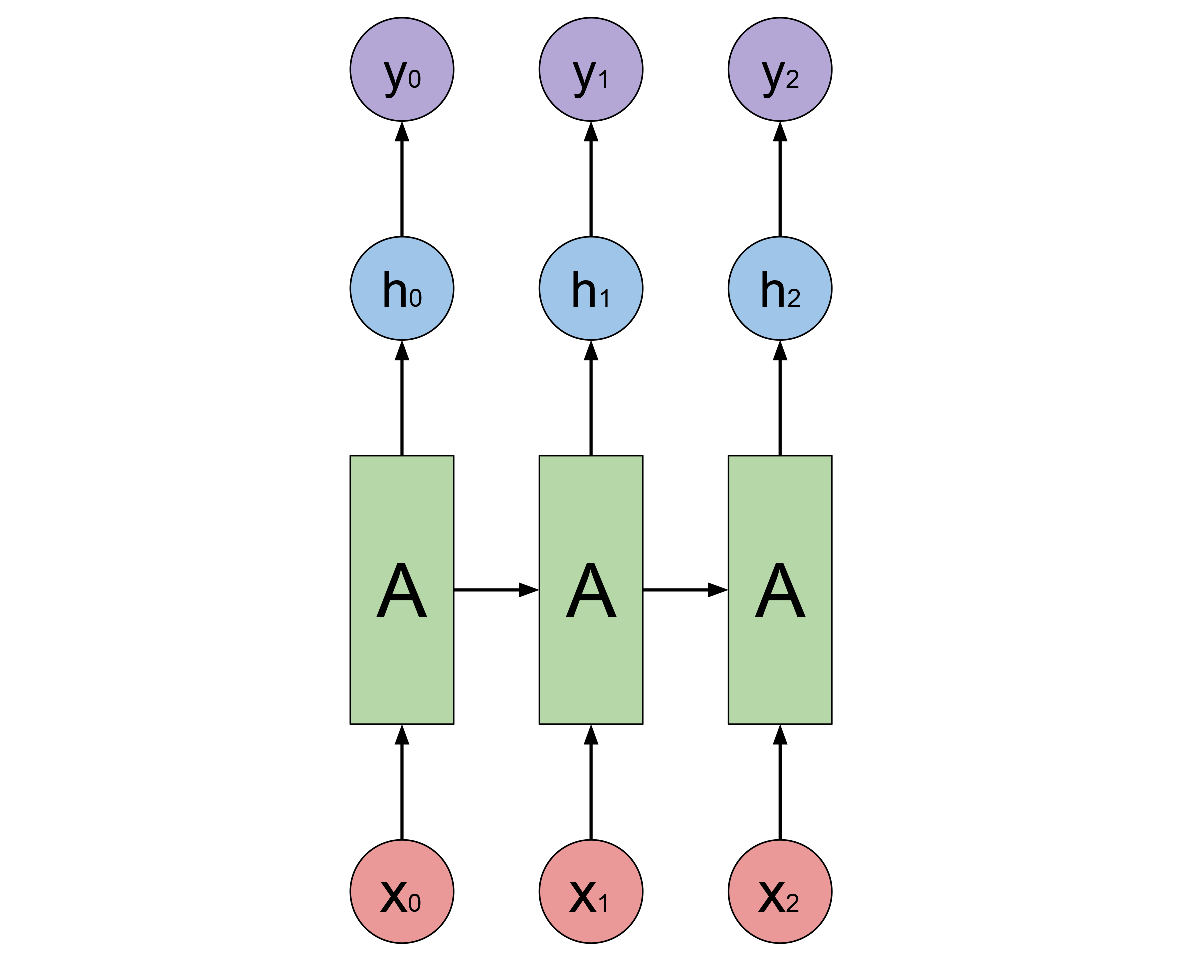
\includegraphics[height=0.2\textwidth]{images/many_to_many.pdf}\end{center} \\
% \hline
% This is some text & \begin{center}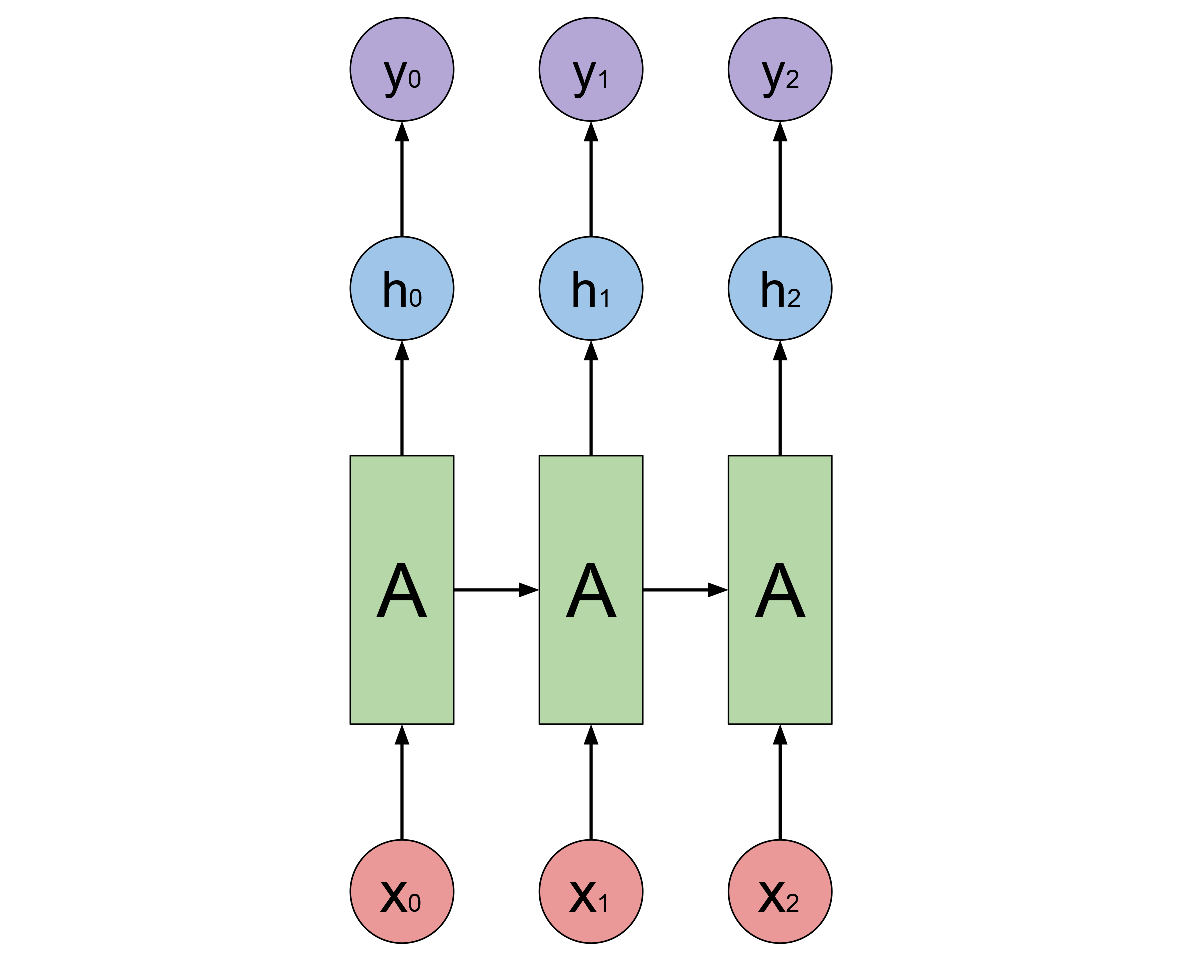
\includegraphics[height=0.2\textwidth]{images/many_to_many.pdf}\end{center} & & \\
% \hline
% \end{tabular}
% \label{tab:gt}
% \end{table}

% \begin{itemize}
%     \item One-to-One if $l_x = l_y = 1$, this is a traditional neural network;
%     \item One-to-Many if $l_x = 1, l_y > 1$, this is the case for sequence generation;
%     \item Many-to-One if $l_x > 1, l_y = 1$, for sequence classification;
%     \item Many-to-Many if $l_x = l_y > 1$, for sequence labeling;
%     \item Many-to-Many if $l_x \neq l_y, l_x > 1, l_y > 1$, for sequence to sequence tasks.
% \end{itemize}

We can also have bidirectional RNN~\citep{Schuster1997birnn} (biRNN), which is composed of two RNNs, one looks at the sequence starting from the end while the other from the beginning as usual. The output at each step of a bidirectional RNN is the concatenation of the hidden states for that time step. In a biRNN we have a left-to-right hidden state (or forward state) $\overrightarrow{h_t} = RNN(x_t, \overrightarrow{h}_{t-1})$, a right-to-left one (or backward state) $\overleftarrow{h_t} = RNN(x_t, \overleftarrow{h}_{t-1})$, and the output hidden state $h_t$ is defined as the concatenation of the directional hidden layers: $h_t = [\overrightarrow{h_t}, \overleftarrow{h_t}]$. The advantage of having bidirectional information is quite clear, the model is able to represent also future information, so the current decision is affected by both past and future.

Recurrent networks have various advantages over traditional networks. These include the ability to process sequences of any length, the size of the model does not increase with the size of the input, and the most important, the computation takes into consideration historical information that should allow RNNs to learn long-term dependencies. Unfortunately, they also have some drawbacks; they are computationally more intensive. Moreover, even if they can work with a sequence of any length and pass information through time, this information transfer starts to become less effective for longer sequences, which means they struggle to model long-term dependencies. That is caused by the vanishing/explosion of the gradient, a significant issue in vanilla RNN. 

The vanishing gradient problem was first studied by~\cite{Hochreiter:91} and ~\cite{bengio1994vanishing}. The problem occurs when we try to train a neural network model using gradient-based optimisation techniques, the backpropagation of the loss function with respect to the weights tends to vanish. This is a consequence of what happens during forward propagation; the hidden state is multiplied several times with the weight matrix, once per time step. So, during backpropagation, this leads to the gradients being multiplied by the same values many times, causing the values to either explode, i.e. grow extremely large or vanish, i.e. become very small, making the model unable to learn. In RNNs this translates to that is very tough to allow the error to flow from the later in time inputs to the ones at the beginning, thus creating difficulties to train the early stages of the RNN and reducing the ability to learn long-term dependencies due to insufficient weight changes.

% \begin{equation}
% \begin{split}
%     h_t & = tanh(W_{h} * h_{t-1} + W_x * x_t) \\
%     y_t & = W_y * h_t
% \end{split}
% \end{equation}

% \begin{figure*}[ht!]
%     \centering
%     \begin{subfigure}[t]{0.3\textwidth}
%         \centering
%         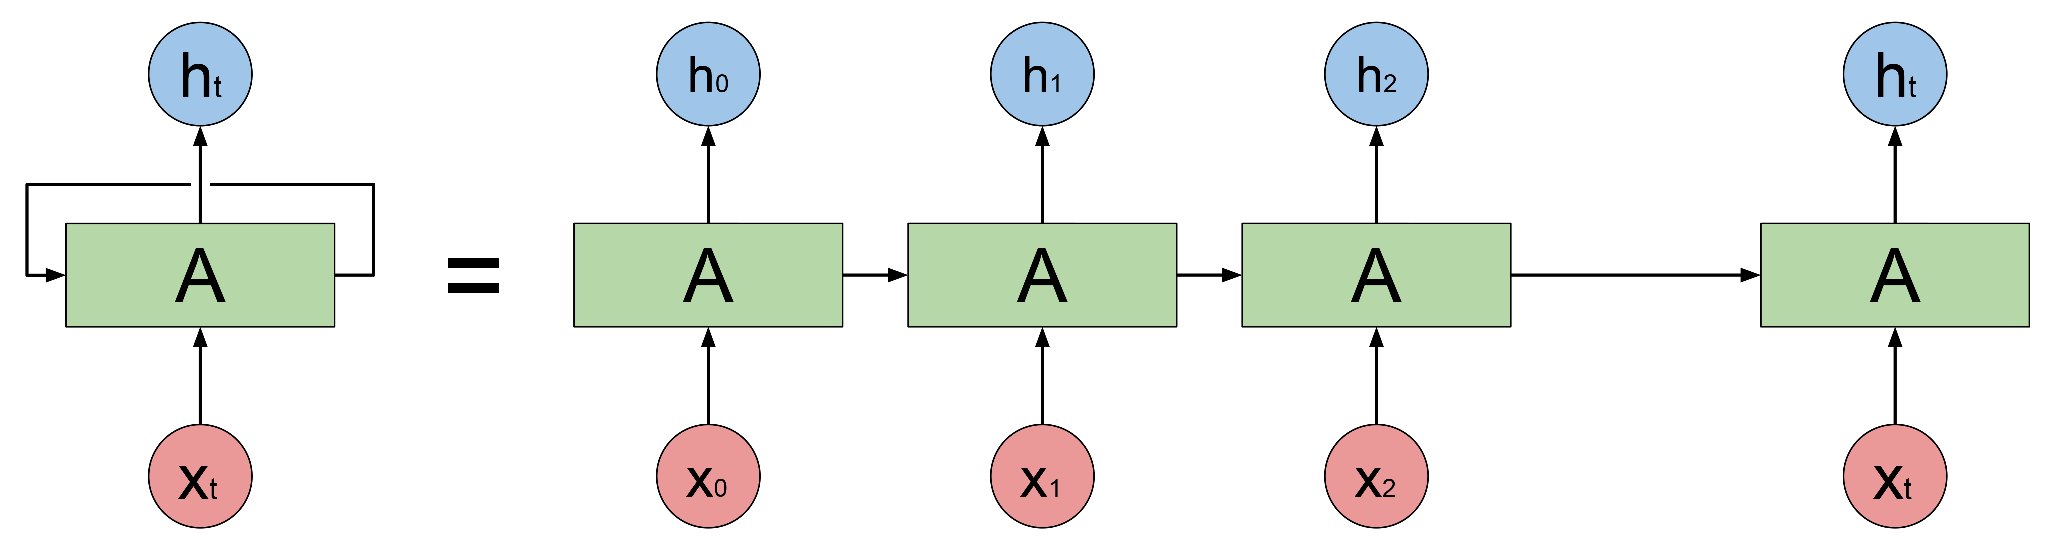
\includegraphics[width=0.7\textwidth]{images/RNN.png}
%         \caption{}
%         \label{subfig:rnn}
%     \end{subfigure}%
%     ~ 
%     \begin{subfigure}[t]{0.7\textwidth}
%         \centering
%         \includegraphics[width=\textwidth]{images/RNN-unrolled_only.png}
%         \caption{}
%         \label{subfig:rnn_unrolled}

%     \end{subfigure}
%     \caption{Different views of a recurrent neural network. In Figure~\ref{subfig:rnn} we have the compact view. Figure~\ref{subfig:rnn_unrolled} shows the same architecture but unrolled. Image credit: Christopher Olah}
%     \label{fig:rnn}
% \end{figure*} 


\subsection{Long Short Term Memory}
\label{sec:lstm}

\begin{figure}[]
    \centering
    \begin{subfigure}[t]{0.5\textwidth}
        \centering
        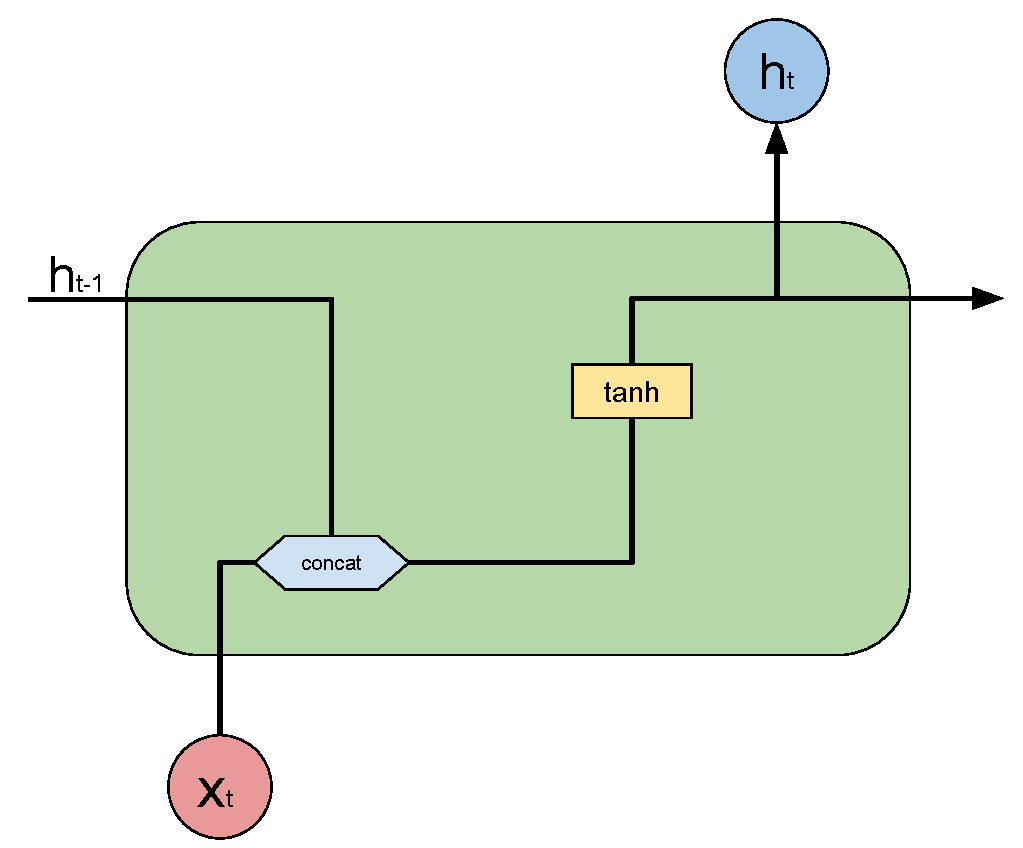
\includegraphics[width=\textwidth]{images/RNN_cell_simple.pdf}
        \caption{Vanilla RNN cell}
        \label{subfig:rnn_cell}

    \end{subfigure}%
    ~ 
    \begin{subfigure}[t]{0.5\textwidth}
        \centering
        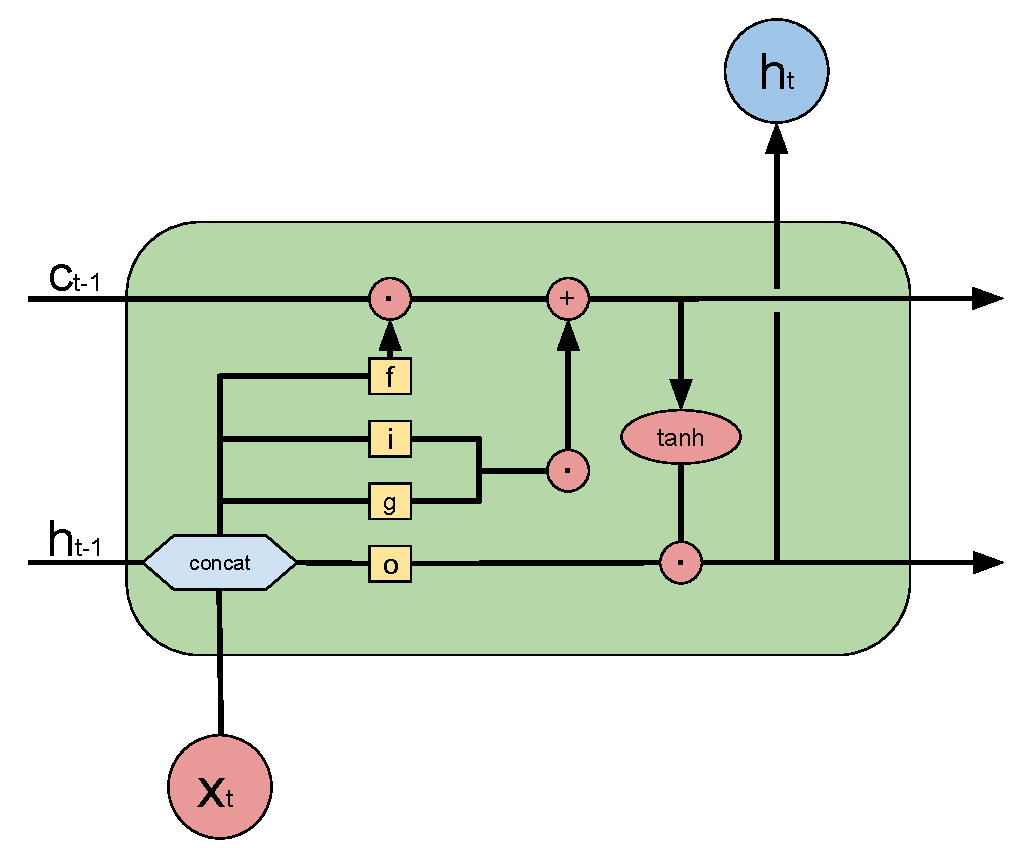
\includegraphics[width=\textwidth]{images/LSTM_cell_simple.pdf}
        \caption{LSTM cell}
        \label{subfig:lstm_cell}

    \end{subfigure}
    \caption{Different types of cells. Red circles are for point-wise operations, in yellow we have neural networks.} % activation functions (these can be seen as neural network, where the weights are in W, and they use different parts of W). } % The blue circle is the dot product, and the stack operation creates a n-dimensional vector with n as the number of input elements.}
    \label{fig:cells}
\end{figure} 

\paragraph{}
Long Short Term Memory networks (LSTM) are an improved version of RNN  that introduces mechanisms to decide what should be ``remembered'' and ``forgotten''. Proposed by~\cite{hochreiter1997long}, LSTMs are a solution to the long-term dependencies issue in vanilla RNN and the vanishing of the gradient. LSTMs mitigate the problem by having a more complex cell that contains two hidden states. The first one is $h_t$ and is similar to the one in RNNs, the other is $C_t$, the cell state, which is the core of a LSTM cell. The cell state is modified using the gates, which are neural networks acting on the information of the cell state and the hidden state. In Figure~\ref{fig:cells} we can see how the information flows and interact with the different gates, these are:

\begin{itemize}
    \item Forget gate layer ($f$): acts on what and how much to forget from the previous time step. It is computed using a neural network with a sigmoid $\sigma$ activation function. The output of the network is between 0 and 1, since the output will be multiplied element-wise 0 means forget all, and 1 remember all. $f_t = \sigma(W_f * [h_{t-1}, x_t])$;
    \item Input gate layer ($i$): this gate decides which information to write to the cell state. It is a sigmoid layer: $i_t = \sigma(W_i * [h_{t-1}, x_t])$, and works in combination with the gate layer; 
    \item Gate gate layer ($g$): decides how much to write to the cell state. It is a $\tanh$ layer, $g_t = \sigma(W_g * [h_{t-1}, x_t])$. The output is the multiplied by the input gate output to create a new candidate state cell that will be summed with the value of the previous cell state after the forget step. The new cell state is  $c_t & = f_t \odot c_{t-1} + i_t \odot g_t$;
    \item Output gate layer ($o$): this layer is responsible of how much of the cell state to reveal through the hidden state. This is done using a sigmoid layer which decides the parts of the cell state that will be shown in the output, formally $o_t = \sigma(W_o * [h_{t-1}, x_t])$. Then, we put the cell state through $\tanh$ (to push the values to be between −1 and 1) and multiply it by the output of the output layer, so that we only expose the parts we decided to. Formally, the hidden state will be $h_t & = o_t \odot \tanh(c_t)$.
    
\end{itemize}


% The previous equations can be wrote more compactly as show in Equation~\ref{eq:lstm}. We have $W \in \mathbb{R}^4$, where each element is a matrix of weights for the different layers of the cell. The hidden layer $h_t$ and the input $x_t$ are both vectors. And $\sigma$, $tahn$ are the activation functions. 

% \begin{equation}
% \begin{split}
%          W & = [W_i, W_f, W_o, W_g] \\ 
%          \begin{bmatrix}
%           i \\
%           f \\
%           o \\
%           g   
%         \end{bmatrix} & =         \begin{bmatrix}
%           \sigma \\
%           \sigma \\
%           \sigma \\
%           \tanh
%          \end{bmatrix}  W   \left[ h_{t-1}, x_t\right]\\
%          c_t & = f \odot c_{t-1} + i \odot g \\
%          h_t & = o \odot \tanh(c_t) \\
% \end{split}
% \label{eq:lstm}
% \end{equation}

This is the general LSTM; however there are many variants of LSTMs, which perform slightly better or worse depending on the task. A more detailed work on how each variant perform is ``LSTM: A Search Space Odyssey'' by~\citet{greff2017lstm}.


\subsection{Attention mechanism}



\paragraph{}
A very popular RNN architecture is the sequence to sequence, or encoder-decoder ~\citep{cho-etal-2014-learning,sutskever2014sequence}. This framework is used in neural machine translation, text summarization, question answering, and many more. 
% \begin{wrapfigure}{r}{0.5\textwidth}
%         \centering
%         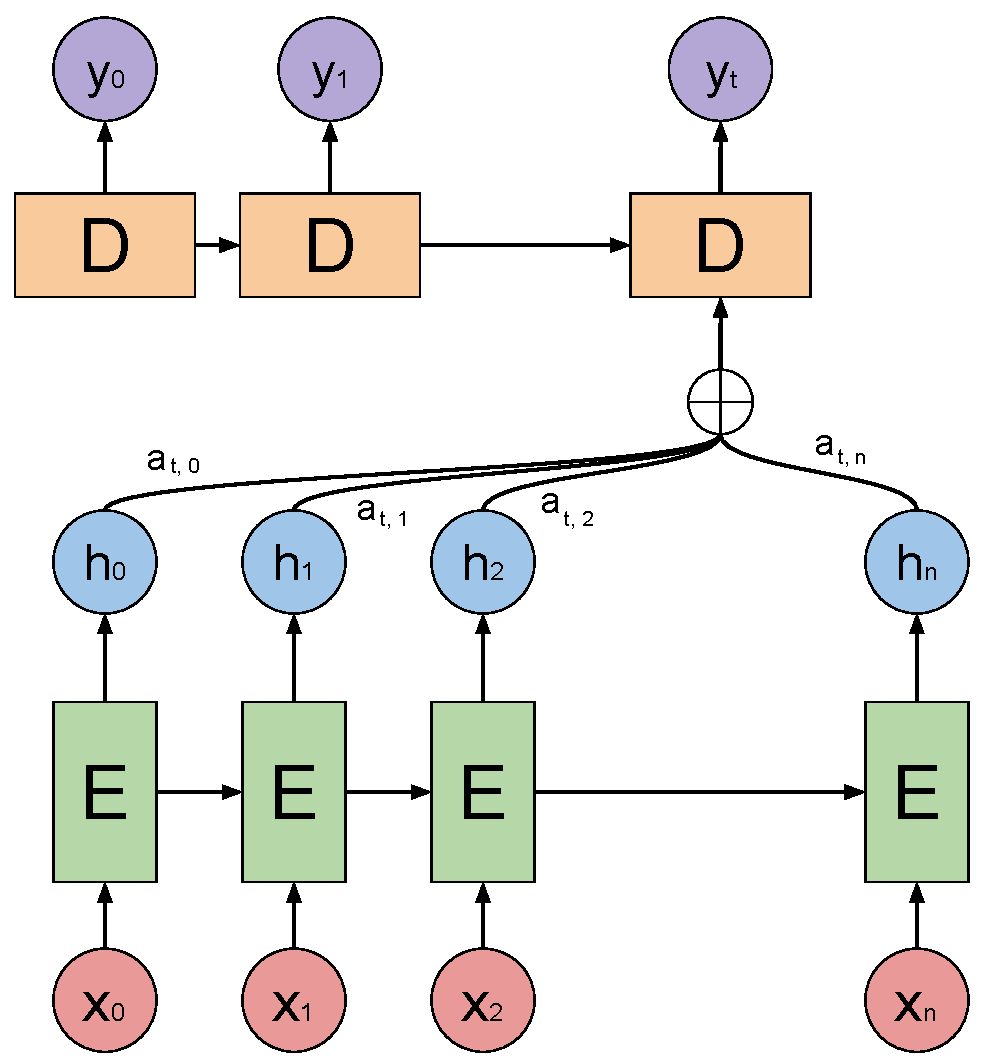
\includegraphics[width=0.5\textwidth]{images/Attention.pdf}
%         \caption{Attention mechanism. The encoder $E$ hidden states are used as input to the decoder $D$ to produce the output of at step $t$.}
%         \label{fig:attention}
% \end{wrapfigure}%

A sequence to sequence model is composed by an encoder, which takes the input sequence and compresses it into a context vector which will be used to start the decoder which predicts a output sequence.  A significant and clear disadvantage of a fixed-length context vector design is as the input sequence get compressed into a single vector, and as this sequence gets longer and longer, more memory is required to store past information. As a result, the network performs poorly o longer sequences~\citep{cho-etal-2014-properties}. A solution to this problem was proposed by~\cite{bahdanau2014neural}, which defines an attention mechanism for the decoder. Instead of just relying on the previous hidden state, the decoder with attention can use the information from all the input sequence by looking at the encoder hidden state at each time step, and combine this information to produce the output.

\paragraph{Encoder:} Given a sequence of vectors $\textbf{x} = (x_1, \dots, x_n)$, an RNN takes this sequence and produces a context vector $c$:

\begin{equation}
    \begin{split}
        h_t & = f(x_t, h_{t-1})\\
        c & = q(\{h_1, \dots, h_n\}) 
    \end{split}
\end{equation}

where $h_t$ is the hidden state at time $t$, and $f$ and $q$ are nonlinear functions. Some example of $f$ and $g$ include: LTSMs for $f$, and return the last hidden state for $g$. This part is the same with or without attention mechanism.

\begin{figure}[t]
        \centering
        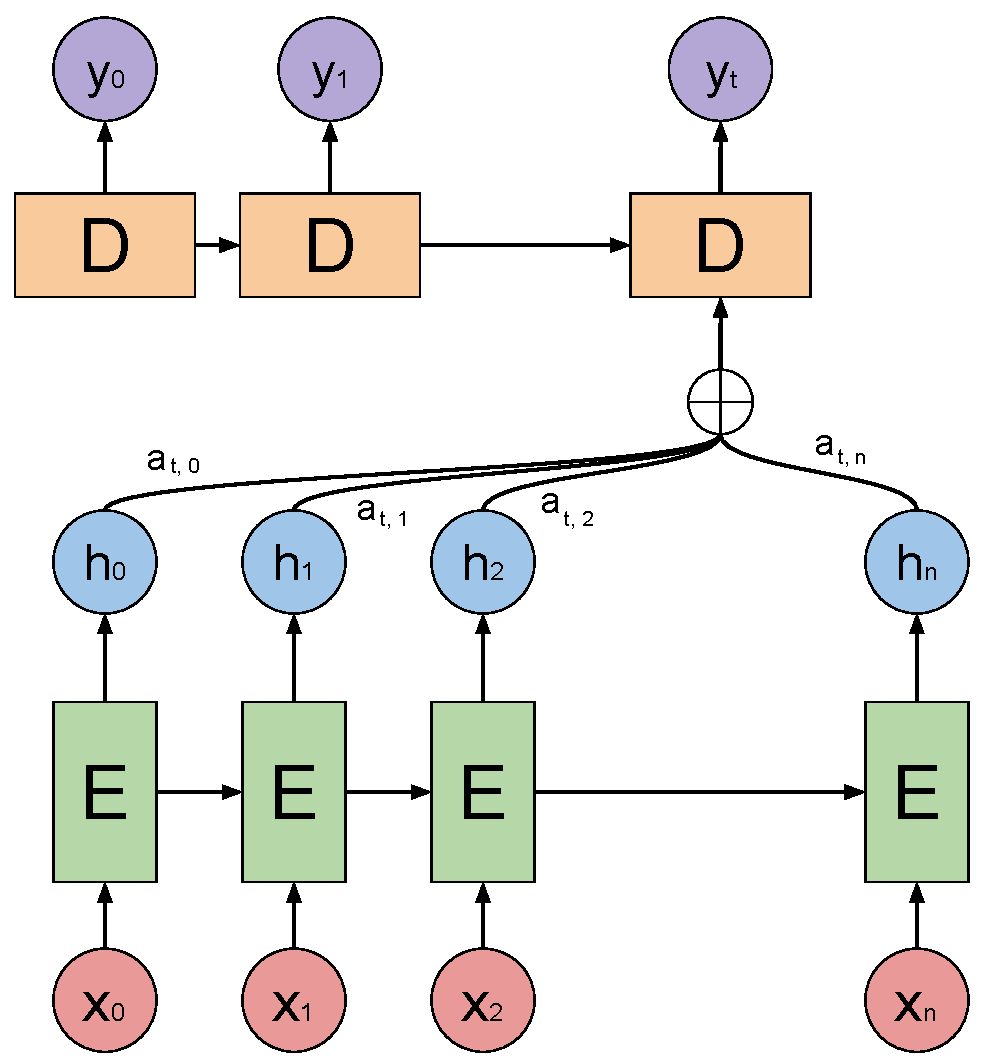
\includegraphics[width=0.5\textwidth]{images/Attention.pdf}
        \caption{Attention mechanism. The encoder $E$ hidden states are weighted via $a_{i, j}$, summed, and used as input to the decoder $D$ to produce the output at step $t$.}
        \label{fig:attention}
\end{figure}%

\paragraph{Decoder:} Given a context vector, the decoder computes the probability of a sequence $\textbf{y} = (y_1, \dots, y_T)$ by decomposing the joint probability into the ordered conditionals to the context vector, and the previous outputs.

\begin{equation}
p(\mathbf{y})=\prod_{t=1}^{T} p\left(y_{t} |\left\{y_{1}, \cdots, y_{t-1}\right\}, c\right)
\end{equation}

Which can be implemented using RNNs, where $g$ is a nonlinear function, and $s_t$ is the decoder hidden state:

\begin{equation}
p(\mathbf{y})=\prod_{t=1}^{T} g\left(y_{t-1}, s_{t}, c\right)
\end{equation}

\paragraph{Decoder with Attention:} Illustrated in Figure~\ref{fig:attention}, the \cite{bahdanau2014neural} decoder performs the same task as the before, but instead of being conditioned to the context vector and the previous output, the probability of each output is conditioned to the previous outputs, and the entire input sequence.


\begin{equation}
p(\mathbf{y})=\prod_{t=1}^{T} p\left(y_{t} |\left\{y_{1}, \cdots, y_{t-1}\right\}, \textbf{x}\right) = \prod_{t=1}^{T} g\left(y_{t-1}, s_{t}, c_t\right)
\end{equation}

The new context vector is computed as a weighted sum of the encoder hidden state $(h_1, \dots, h_n)$: 

\begin{equation}
\begin{split}
    c_{i} & = \sum_{j=1}^{n} \alpha_{i j} h_{j}\\
    \alpha_{i j} &= \frac{\exp \left(e_{i j}\right)}{\sum_{k=1}^{T_{x}} \exp \left(e_{i k}\right)} \\
    e_{i j} &= a\left(s_{i-1}, h_{j}\right)
\end{split}
\end{equation}

The weight $\alpha_{i j}$ is a probability that indicates the importance of the $j$-th encoder state $h_j$ with regard to the previous decoder hidden state $s_{i-1}$ to produce the next hidden state $s_i$ and the output of $y_i$ . The weights are computed using a neural network $a$ called alignment model, since~\cite{bahdanau2014neural} proposed this architecture in a neural machine translation task. Having the decoder look at the entire input sequence implements a so-called attention mechanism, which allows the encoder to decide at which part of the input to attend.  By letting the decoder have an attention mechanism, we reduce the encoder responsibility of having to encode all information in the source sequence into a fixed length vector since the decoder can selectively retrieve the useful information in the sequence accordingly to the current state needs.

The idea of having an attention mechanism become very successful in many other NLP task due to the increase in performance it brings. This value in NLP inspired a new model, called Transformer~\citep{vaswani2017attention}, entirely based on it. 

\subsection{Transformer}

\section{Word Representation}
\label{sec:word_embedding}
\paragraph{}
Word representation is an elemental part of most Natural Language Processing (NLP) tasks. The understanding of text is mainly derived by transforming text to usable computational representations, these include graphs, trees, or vectors on which will the focus.   In general, it has been found to be beneficial to represent words or documents as vectors, which have an appealing, intuitive interpretation, and they capture hidden information concerning a language, like word analogies or semantic. 
%A word representation is a mathematical object associated with each word, often a vector.

% Based on the literature \citep{turian2010word, schnabel2015embeddings},  \cite{almeida2019word} define word embeddings as a e dense, distributed, fixed-length word vectors, built using word co-occurrence statistics as per the distributional hypothesis

There are various methods to induce word representation:

\begin{itemize}[itemsep = 0.1em]
\item Distributional word representation: are based on co-occurrence context and on the distributional hypothesis:  ``\textit{linguistic items with similar distributions have similar meanings}'', hence the similarity is expressed in terms of the similarity of the distribution. Some common representation techniques include Latent Semantic Analysis~\citep{deerwester1990indexing} and Latent Dirichlet Allocation~\citep{bei2003lda, das-etal-2015-gaussian}. An important example is the work of \citet{pennington2014glove} which propose a competitive set of pre-trained word representations, his work signals that word representation had reached the main stream.

\item Distributed representation: are compact, dense and low dimensional representation, where each dimension of the embedding represents a latent feature of the word, hopefully capturing useful syntactic and semantic properties. A distributed representation is compact, in the sense that it can represent an exponential number of clusters in the number of dimensions. Some examples include the work of \citet{Collobert2008} which for the first time demonstrated the utility of word embeddings for downstream tasks and their proposed neural network architecture forms the foundation for many current approaches, and the Word2Vec framework proposed by \citet{mikolov2013distributed} which popularized word embeddings.
\end{itemize}

In the work ``\textit{Word representations: A simple and general method for semi-supervised learning}'', \citet{turian2010word} define as ``\textit{word embeddings}'' only the distributed representation, but over time this distinction is not enforced and is common to refer to all vector word representations as word embeddings.


\paragraph{}
Another essential part of NLP is the study of language models. A language model is a statistical model of language usage. It consists mainly of predicting the next word given some previous words. A language model learns the probability of word occurrence based on examples of text. Simpler models may look at a context of a short sequence of words, whereas larger models may work at the level of sentences or paragraphs.

More formally, the goal of a statistical language model is to learn the probability $P(x_1, \dots, x_m)$ for a sequence of tokens $x_1, \dots, x_m$. We can compute this via the chain rule of probability:

\begin{equation}
P\left(w_{1}, \ldots, w_{m}\right)=\prod_{i=1}^{m} P\left(w_{i} | w_{1}, \dots, w_{i-1}\right)
\end{equation}

Because the number of words that precede a word varies, and because it is difficult to compute $P(w_i | w_1,\dots, w_{i-1})$ with $i$ large, we typically condition the probability of a word on a window of n previous words ($n$-grams): 


\begin{equation}
P\left(w_{1}, \ldots, w_{m}\right) \approx \prod_{i=1}^{m} P\left(w_{i} | w_{i-n}, \dots, w_{i-1}\right)
\end{equation}

This approach doesn't generalize to new sequences, unless using some tricks like~\citet{katz1987probablm} did where he computes small $n$-grams, generally $n=3$, and then generalizes to unseen sequences by producing new ones using overlapping n-grams of length up to $n$. However, this solution does not generalize to sequences longer than $n$, which has to be small, and also does not take in consideration the similarities of words. Moreover, statistical language models suffer from the problem known as curse of dimensionality that appears when the vocabulary size increases. For example, computing the joint probability of 10 consecutive words having a vocabulary size of 100k there are $100000^{10} - 1 = 10^{50} - 1$ free parameters. 

\citet{bengio2000nnlm} developed a solution for the course of dimensionality of statistical language models by proposing the first large-scale language model based on neural networks, referred to as Neural Network Language Models (NNLMs). In their work \citet{bengio2000nnlm} bring together language modeling and word embeddings by \begin {enumerate*} [1) ]%
\item associating each word in the vocabulary with a distributed word vector called ``\textit{feature vector}'' \item express the joint probability function of word sequences in terms of the feature vectors of these words in the sequence; \item learn simultaneously the word feature vector and the parameters of the probability function.
\end {enumerate*} This new representation also generalizes to longer sequences and is able to learn similarities between words. \citet{bengio2000nnlm} conclude their work by suggesting the use of Recurrent Neural Networks (RNN) to take advantage of temporal structures and also consider longer sequences like entire paragraphs.

A few years later, \citet{Mikolov2010RecurrentNN} propose a neural language model based on RNN. They use a vanilla RNN~\citep{elman1990finding} to show how language models based on recurrent networks are significantly better that previous solution. They perform experiments on various speech recognition task, and achieve better results even when training using lower amount of data.

This work and the one of \cite{bengio2000nnlm} were followed by many other word embeddings solutions that build upon their methods, in particular current state of the art use RNN, or improved versions like Long Short Term Memory networks~\citep{hochreiter1997long}. We will now present in more detail some of these works using the following architectures: GloVe~\citep{pennington2014glove}, ELMo~\citep{peters2018elmo},and the two we used in our experiments, BERT~\citep{devlin2018bert} and fastText~\citep{bojanowski2016enriching}.


 % Move fT, and BERT in MODEL

\subsection{fastText}
\subsection{BERT}


\subsection{Multilingual Word Representation}

\section{Transfer Learning}
\label{sec:transfer_learning}
\subsection{Cross-lingual Learning}
\subsection{Multi-task Learning}
 
\section{Zero-Shot, One-Shot and Few Shot Learning} 
\label{sec:zero_learning}

\chapter{State of the Art} % Relation Extraction? | Natural Language Understanding
\label{chpt:3}
\section{Relation Extraction}
\subsection{Zero-Shot Relation Extraction}
\subsection{Multilingual Relation Extraction}

\section{Machine Comprehension}
\subsection{BiDAF}
% \subsection{NAMANDA}